% Created by tikzDevice version 0.12.6 on 2024-03-12 19:53:23
% !TEX encoding = UTF-8 Unicode
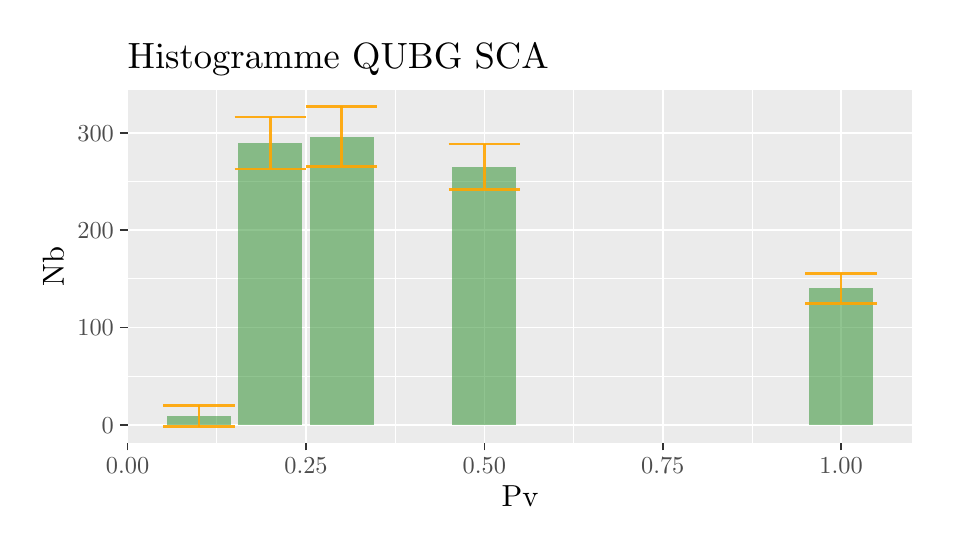
\begin{tikzpicture}[x=1pt,y=1pt]
\definecolor{fillColor}{RGB}{255,255,255}
\path[use as bounding box,fill=fillColor,fill opacity=0.00] (0,0) rectangle (325.21,180.67);
\begin{scope}
\path[clip] (  0.00,  0.00) rectangle (325.21,180.67);
\definecolor{drawColor}{RGB}{255,255,255}
\definecolor{fillColor}{RGB}{255,255,255}

\path[draw=drawColor,line width= 0.6pt,line join=round,line cap=round,fill=fillColor] (  0.00,  0.00) rectangle (325.21,180.68);
\end{scope}
\begin{scope}
\path[clip] ( 36.11, 30.69) rectangle (319.71,158.02);
\definecolor{fillColor}{gray}{0.92}

\path[fill=fillColor] ( 36.11, 30.69) rectangle (319.71,158.02);
\definecolor{drawColor}{RGB}{255,255,255}

\path[draw=drawColor,line width= 0.3pt,line join=round] ( 36.11, 54.69) --
	(319.71, 54.69);

\path[draw=drawColor,line width= 0.3pt,line join=round] ( 36.11, 89.90) --
	(319.71, 89.90);

\path[draw=drawColor,line width= 0.3pt,line join=round] ( 36.11,125.11) --
	(319.71,125.11);

\path[draw=drawColor,line width= 0.3pt,line join=round] ( 68.34, 30.69) --
	( 68.34,158.02);

\path[draw=drawColor,line width= 0.3pt,line join=round] (132.79, 30.69) --
	(132.79,158.02);

\path[draw=drawColor,line width= 0.3pt,line join=round] (197.25, 30.69) --
	(197.25,158.02);

\path[draw=drawColor,line width= 0.3pt,line join=round] (261.71, 30.69) --
	(261.71,158.02);

\path[draw=drawColor,line width= 0.6pt,line join=round] ( 36.11, 37.08) --
	(319.71, 37.08);

\path[draw=drawColor,line width= 0.6pt,line join=round] ( 36.11, 72.29) --
	(319.71, 72.29);

\path[draw=drawColor,line width= 0.6pt,line join=round] ( 36.11,107.51) --
	(319.71,107.51);

\path[draw=drawColor,line width= 0.6pt,line join=round] ( 36.11,142.72) --
	(319.71,142.72);

\path[draw=drawColor,line width= 0.6pt,line join=round] ( 36.11, 30.69) --
	( 36.11,158.02);

\path[draw=drawColor,line width= 0.6pt,line join=round] (100.57, 30.69) --
	(100.57,158.02);

\path[draw=drawColor,line width= 0.6pt,line join=round] (165.02, 30.69) --
	(165.02,158.02);

\path[draw=drawColor,line width= 0.6pt,line join=round] (229.48, 30.69) --
	(229.48,158.02);

\path[draw=drawColor,line width= 0.6pt,line join=round] (293.93, 30.69) --
	(293.93,158.02);
\definecolor{fillColor}{RGB}{34,139,34}

\path[fill=fillColor,fill opacity=0.50] ( 50.29, 37.08) rectangle ( 73.50, 40.32);

\path[fill=fillColor,fill opacity=0.50] ( 76.07, 37.08) rectangle ( 99.28,139.02);

\path[fill=fillColor,fill opacity=0.50] (101.86, 37.08) rectangle (125.06,141.33);

\path[fill=fillColor,fill opacity=0.50] (153.42, 37.08) rectangle (176.62,130.43);

\path[fill=fillColor,fill opacity=0.50] (282.33, 37.08) rectangle (305.53, 86.42);
\definecolor{drawColor}{RGB}{255,165,0}

\path[draw=drawColor,draw opacity=0.90,line width= 0.9pt,line join=round] ( 49.00, 44.17) --
	( 74.78, 44.17);

\path[draw=drawColor,draw opacity=0.90,line width= 0.9pt,line join=round] ( 61.89, 44.17) --
	( 61.89, 36.47);

\path[draw=drawColor,draw opacity=0.90,line width= 0.9pt,line join=round] ( 49.00, 36.47) --
	( 74.78, 36.47);

\path[draw=drawColor,draw opacity=0.90,line width= 0.9pt,line join=round] ( 74.78,148.37) --
	(100.57,148.37);

\path[draw=drawColor,draw opacity=0.90,line width= 0.9pt,line join=round] ( 87.68,148.37) --
	( 87.68,129.68);

\path[draw=drawColor,draw opacity=0.90,line width= 0.9pt,line join=round] ( 74.78,129.68) --
	(100.57,129.68);

\path[draw=drawColor,draw opacity=0.90,line width= 0.9pt,line join=round] (100.57,152.23) --
	(126.35,152.23);

\path[draw=drawColor,draw opacity=0.90,line width= 0.9pt,line join=round] (113.46,152.23) --
	(113.46,130.43);

\path[draw=drawColor,draw opacity=0.90,line width= 0.9pt,line join=round] (100.57,130.43) --
	(126.35,130.43);

\path[draw=drawColor,draw opacity=0.90,line width= 0.9pt,line join=round] (152.13,138.65) --
	(177.91,138.65);

\path[draw=drawColor,draw opacity=0.90,line width= 0.9pt,line join=round] (165.02,138.65) --
	(165.02,122.20);

\path[draw=drawColor,draw opacity=0.90,line width= 0.9pt,line join=round] (152.13,122.20) --
	(177.91,122.20);

\path[draw=drawColor,draw opacity=0.90,line width= 0.9pt,line join=round] (281.04, 91.84) --
	(306.82, 91.84);

\path[draw=drawColor,draw opacity=0.90,line width= 0.9pt,line join=round] (293.93, 91.84) --
	(293.93, 81.01);

\path[draw=drawColor,draw opacity=0.90,line width= 0.9pt,line join=round] (281.04, 81.01) --
	(306.82, 81.01);
\end{scope}
\begin{scope}
\path[clip] (  0.00,  0.00) rectangle (325.21,180.67);
\definecolor{drawColor}{gray}{0.30}

\node[text=drawColor,anchor=base east,inner sep=0pt, outer sep=0pt, scale=  0.88] at ( 31.16, 34.05) {0};

\node[text=drawColor,anchor=base east,inner sep=0pt, outer sep=0pt, scale=  0.88] at ( 31.16, 69.26) {100};

\node[text=drawColor,anchor=base east,inner sep=0pt, outer sep=0pt, scale=  0.88] at ( 31.16,104.48) {200};

\node[text=drawColor,anchor=base east,inner sep=0pt, outer sep=0pt, scale=  0.88] at ( 31.16,139.69) {300};
\end{scope}
\begin{scope}
\path[clip] (  0.00,  0.00) rectangle (325.21,180.67);
\definecolor{drawColor}{gray}{0.20}

\path[draw=drawColor,line width= 0.6pt,line join=round] ( 33.36, 37.08) --
	( 36.11, 37.08);

\path[draw=drawColor,line width= 0.6pt,line join=round] ( 33.36, 72.29) --
	( 36.11, 72.29);

\path[draw=drawColor,line width= 0.6pt,line join=round] ( 33.36,107.51) --
	( 36.11,107.51);

\path[draw=drawColor,line width= 0.6pt,line join=round] ( 33.36,142.72) --
	( 36.11,142.72);
\end{scope}
\begin{scope}
\path[clip] (  0.00,  0.00) rectangle (325.21,180.67);
\definecolor{drawColor}{gray}{0.20}

\path[draw=drawColor,line width= 0.6pt,line join=round] ( 36.11, 27.94) --
	( 36.11, 30.69);

\path[draw=drawColor,line width= 0.6pt,line join=round] (100.57, 27.94) --
	(100.57, 30.69);

\path[draw=drawColor,line width= 0.6pt,line join=round] (165.02, 27.94) --
	(165.02, 30.69);

\path[draw=drawColor,line width= 0.6pt,line join=round] (229.48, 27.94) --
	(229.48, 30.69);

\path[draw=drawColor,line width= 0.6pt,line join=round] (293.93, 27.94) --
	(293.93, 30.69);
\end{scope}
\begin{scope}
\path[clip] (  0.00,  0.00) rectangle (325.21,180.67);
\definecolor{drawColor}{gray}{0.30}

\node[text=drawColor,anchor=base,inner sep=0pt, outer sep=0pt, scale=  0.88] at ( 36.11, 19.68) {0.00};

\node[text=drawColor,anchor=base,inner sep=0pt, outer sep=0pt, scale=  0.88] at (100.57, 19.68) {0.25};

\node[text=drawColor,anchor=base,inner sep=0pt, outer sep=0pt, scale=  0.88] at (165.02, 19.68) {0.50};

\node[text=drawColor,anchor=base,inner sep=0pt, outer sep=0pt, scale=  0.88] at (229.48, 19.68) {0.75};

\node[text=drawColor,anchor=base,inner sep=0pt, outer sep=0pt, scale=  0.88] at (293.93, 19.68) {1.00};
\end{scope}
\begin{scope}
\path[clip] (  0.00,  0.00) rectangle (325.21,180.67);
\definecolor{drawColor}{RGB}{0,0,0}

\node[text=drawColor,anchor=base,inner sep=0pt, outer sep=0pt, scale=  1.10] at (177.91,  7.64) {Pv};
\end{scope}
\begin{scope}
\path[clip] (  0.00,  0.00) rectangle (325.21,180.67);
\definecolor{drawColor}{RGB}{0,0,0}

\node[text=drawColor,rotate= 90.00,anchor=base,inner sep=0pt, outer sep=0pt, scale=  1.10] at ( 13.08, 94.35) {Nb};
\end{scope}
\begin{scope}
\path[clip] (  0.00,  0.00) rectangle (325.21,180.67);
\definecolor{drawColor}{RGB}{0,0,0}

\node[text=drawColor,anchor=base west,inner sep=0pt, outer sep=0pt, scale=  1.32] at ( 36.11,166.08) {Histogramme QUBG SCA};
\end{scope}
\end{tikzpicture}
